\chapter{Część serwerowa aplikacji}

Niniejszy rozdział opisuje sposób implementacji części serwerowej projektu RevCommunity. Przedstawiona zostanie warstwowa architektura projektu. Następnie przechodząc przez poszczególne warstwy omówione zostaną technologie wykorzystane do realizacji tej części aplikacji. Przybliżone zostaną również najważniejsze elementy konfiguracji.

\section{Architektura}
W projekcie zastosowano architekturę warstwową opartą na trzech poziomach:

\begin{itemize}
\item Warstwa komunikacji - odpowiada za przetworzenie zapytań klienta i~wywołanie odpowiednich funkcji. Jej zadaniem jest konwersja danych przesłanych w~formacie JSON na obiekty języka Java. Przetworzone dane wejściowe przekazywane są dalej do warstwy biznesowej, która zajmie się realizacją żądanych operacji. Na koniec rezultat wykonanych działań wraca w~odpowiedniej formie do klienta.
\item Warstwa logiki biznesowej - udostępnia funkcje pozwalające zarządzać stanem systemu. Definicje metod odnoszą się do kontekstu biznesowego i~są odseparowane od sposobu realizacji ich zadań. Implementacja, która jest ukryta przed wyższymi warstwami, polega na grupowaniu funkcji dostępu do danych w~logicznie powiązane sekwencje operacji wykonywane w~obrębie jednej transakcji bazodanowej.
\item Warstwa dostępu do danych - zapewnia komunikację z~bazą danych. Interfejsy tej warstwy pozwalają wykonywać operacje CRUD na obiektach encyjnych.
\end{itemize}

Zależności między warstwami są hierarchiczne. Oznacza to, że warstwa wyższa może korzystać wyłącznie z~warstwy bezpośrednio niższej. 
Schemat hierarchii warstw:

\begin{figure}[H]
	\centering
	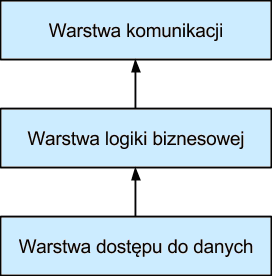
\includegraphics[scale=1]{images/warstwy_serwer.png}
	\caption{Schemat hierarchii warstw}
\end{figure}

Powyższy schemat prezentuje wizualnie zależności między warstwami. Strzałki oznaczają kierunek komunikacji. Warstwa dostępu do danych jest najniżej położona i~nie może korzystać z~żadnej innej warstwy. Poziom logiki biznesowej korzysta z~warstwy dostępu do danych w~celu utrwalenia zmian logiki biznesowej. Warstwa komunikacji nie wie o~istnieniu warstwy dostępu do danych i~nie może się z~nią komunikować. Korzysta wyłączenie z~warstwy niższej, czyli logiki biznesowej.

Dzięki takiej architekturze uzyskano separację grup funkcji co poprawia czytelność, przejrzystość i~ułatwia zarządzanie projektem. Hierarchia zależności znacznie ułatwia wprowadzanie zmian w~projekcie, ponieważ modyfikacja w~jednej warstwie nie wpływa na żadną z pozostałych. Komunikacja między warstwami odbywa się za pośrednictwem interfejsów, a~implementacja jest ukryta. Pozwala to na wykorzystanie konkretnych warstw w~innych projektach.


\section{Warstwa komunikacji}

Do implementacji warstwy komunikacji wykorzystano Spring MVC. Jest to element Spring Framework, pozwalający w~wygodny sposób implementować obsługę zapytań HTTP do serwera. Głównym elementem mechanizmu jest DisptacherServlet, do którego są kierowane wszystkie żądania pasujące do określonego wzorca. Definicja DisptacherServlet znajduje się w~pliku web.xml. Fragment reprezentujący konfigurację może wyglądać następująco:

\begin{figure}[H]
	\centering
	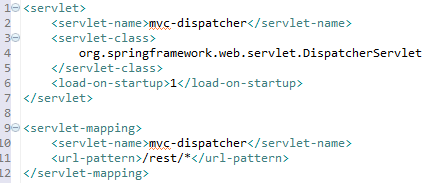
\includegraphics[width=\textwidth]{images/dispatcher.png}
	\caption{Konfiguracja DispatcherServlet}
\end{figure}

Jest to zwykła konfiguracja mapowania servletu. Sprawia ona, że każde żądanie zaczynające się od prefixu /rest/ spowoduje wywołanie DispatcherServlet. Zdaniem tego komponentu jest wykonanie odpowiedniej funkcji obsługującej żądanie. Wymogiem tej techniki jest zdefiniowanie mapowania żądanego adresu URL na odpowiednią klasę i~metodę. Wyszukiwanie dopasowania ogranicza się do klas oznaczonych adnotacją @Controller. Spring MVC filtruje tak oznaczone klasy, a~następnie poszukuje adnotacji @RequestMapping zawierającej informację o~mapowaniu URL na metodę lub klasę. Jeżeli oznaczono klasę adnotacją np. @RequestMapping(“/users”) to wszystkie mapowania metod w~tej klasie będą zaczynały się od “/users”. Przypisując mapowanie do metody wzorzec dopasowania będzie połączeniem ścieżki do klasy i~metody, czyli np. “/users/newest”. Można również zrezygnować z~podawania wzorca przy funkcji, a~zamiast tego dla rozróżnienia operacji określić metodę protokołu HTTP( POST ,GET, PUT, DELETE). Dzięki takiemu podejściu można wywołać zapytanie o~takim samym URL, ale w~zależności użytej metody HTTP wykona się inna operacja. 

Kolejną przydaną funkcją Spring MVC jest bardzo szeroko konfigurowalne konwertowanie parametrów zapytań HTTP na obiekty języka Java. Klasy służące do obsługi zapytań nie muszą implementować żadnego interfejsu, ani rozszerzać żadnej klasy. Są to zwykłe klasy bez specjalnych wymagań poza oznaczeniem adnotacją @Controller. Zatem w~metodach takiej klasy można umieścić argumenty dowolnego typu i~przy minimalnej konfiguracji zmapować parametry zapytania HTTP na odpowiedni typ. Zastosowana technologia udostępnia kilka możliwości realizacji mapowania parametrów. Do dyspozycji są m.in. następujące adnotacje:

\begin{itemize}
\item @RequestParam - umożliwia konwersję parametrów zapytania HTTP na proste typy Java
\item @PathVariable - odczytuje parametry zapytania z~adresu URL. Pozwala na zastosowanie schematu REST 
\item @RequestBody - umożliwia mapowanie obiektu javascript na złożony obiekt Java. Wymaga odpowiedniego ustawienia nagłówków zapytania HTTP
\end{itemize}

Można również, jako argument, podać obiekt pewnej klasy bez żadnej adnotacji. W takim przypadku jeżeli nazwa pola tej klasy zgadza się z~nazwą parametru zapytania, to do tego pola wpisana zostanie wartość parametru. Bez umieszczania adnotacji można również podać pewne standardowe parametry np. HttpServletRequest, HttpServletResponse, czy HttpSession{cite{springmvcWww}.

W projekcie zastosowano wzorzec REST do stworzenia struktury mapowań żądań HTTP na metody odpowiednich klasy. Wzorzec ten wprowadza pojęcie zasobu, który możemy jednoznacznie zidentyfikować poprzez powiązany z~nim identyfikator. To podejście różni się od klasycznego tym, że parametry przekazujemy w~adresie URL, a~nie w~treści zapytania. Wzorzec narzuca pewne zasady konstruowania API umożliwiającego zarządzanie zasobami. Adres URL rozpoczyna się od identyfikatora grupy zasobów np. “/users” określa, że operacje dotyczą użytkowników. Duże znaczenie mają metody protokołu HTTP, ponieważ każda będzie oznaczać inną operację. Jeżeli nie podano identyfikatora konkretnego zasobu(np. ID użytkownika), czyli adres naszego zapytania to “/users”, to w~zależności od metody HTTP powinny wykonać się następujące operacje:

\begin{itemize}
\item GET - pobiera listę wszystkich zasobów (np. listę użytkowników)
\item POST - tworzy nowy zasób (np. nowego użytkownika)
\item PUT - zastępuje wszystkie zasoby
\item DELETE - usuwa wszystkie zasoby
\end{itemize}

Gdy do adresu zostanie dodany identyfikator zasobu np. “users/23” odwołania będą dotyczyć konkretnego zasobu i~API powinno udostępniać metody:

\begin{itemize}
\item GET - pobranie zasobu o~podanym id
\item POST - traktuje wskazany zasób jako kolekcję i~dodaje do niej przekazany jako parametr zasób
\item PUT - modyfikacja zasobu
\item DELETE - usunięcie zasobu
\end{itemize}

Oczywiście API nie ogranicza się tylko do powyżej opisanych metod. Prezentuje tylko podstawowe schematy mapowania żądań na operacje. Jeżeli np. na obiekcie użytkownika ma wykonać się pewna specyficzna operacja, np. dezaktywacja, to należy dodać po jego id, nazwę akcji, która ma zostać wywołana na tym zasobie np.: “users/23/deactivate”. 
W praktyce często między zasobami istnieją powiązania, do których również można się odwoływać w~sposób zgodny ze architekturą REST. Przykładowo w~projekcie RevCommunity istnieją powiązania użytkowników(autorów) i~recenzji. W celu pobrania listy recenzji danego autora można wywołać zapytanie “reviews/user/23”.
Przy korzystaniu z~architektury REST mogą pojawić się pewne problemy, gdy w~zapytaniu HTTP  przesyłane jest wiele parametrów, lub ich rozmiar jest bardzo duży. W takim przypadku wygenerowanie odpowiedniego URL może stać się dużo bardziej kłopotliwe niż zastosowanie standardowych parametrów lub przesłanie obiektu javascript w~formacie JSON. Operacja wyszukiwania może posłużyć jako przykład, w~którym lepsze okazuje się klasyczne podejście. W systemie można wyszukiwać produkty podając ich specyficzne parametry np. producenta, wymiary, etc. Ilość parametrów po których można filtrować wyniki nie jest ograniczona. Trudno sobie wyobrazić jak miałby wyglądać URL wygenerowany na podstawie takich parametrów pamiętając o architekturze REST. Kolejną bardzo istotną sprawą jest fakt, iż długość adresu URL jest ograniczona w~najpopularniejszych przeglądarkach do około 2000 znaków. Serwer do którego wysyłane jest zapytanie również może mieć pewne limity długości zapytania. Dlatego wykorzystanie metody POST w~tradycyjny sposób wydaje się być dużo lepszym rozwiązaniem. Oczywiście metoda POST również ma ograniczenia co do rozmiaru, jednak jest to wartość rzędu 2MB, którą dużo trudniej w~praktyce przekroczyć\cite{restWww}.

Spring MVC poza mapowaniem parametrów wejściowych zapytań HTTP umożliwia również konwersję zwracanych danych do różnych formatów, lub przekierowanie do odpowiedniego widoku. Warstwa prezentacji projektu RevCommunity działa w~sposób dynamiczny, czyli nie jest odświeżana cała strona podczas przejścia między widokami, lecz zmieniane są dynamicznie wyświetlane treści. To znacznie ograniczyło wykorzystywanie przekierowań do widoków w~kontrolerach, na rzecz konwersji danych do formatu JSON. Spring MVC pozwala na konwersję do wielu innych formatów m.in. XML, obraz, strumień bajtów, łańcuch znaków. Jednak w tym przypadku kontrolery zgodnie z~ideą REST zwracają pewne zbiory danych(zasobów) bez informacji o~wyglądzie tych danych(wygląd zaimplementowany jest w~części klienckiej). Dobrym wyborem w~takiej sytuacji wydaje się również XML jednak format JSON jest częścią języka javascript co znaczeni uprościło komunikację między serwerem, a~klientem( część kliencka oparta jest głównie o~język javascript).
Czym tak naprawdę jest JSON? JSON(JavaScript Object Notation) jest to format służący do przechowywania i~wymiany danych. Podobnie jak XML format JSON ma strukturę drzewiastą i~jest wspierany przez technologię AJAX. Każdy z~formatów ma wady i~zalety. Format XML wymaga więcej miejsca, ze względu na znaczniki przy każdej wartości i~znaczniki końcowe, jednak z~drugiej strony zwiększa to czytelność dokumentu. Przykładowo mając długą listę elementów w~dokumencie XML w~dowolnym miejscu widoczny jest znacznik opisujący wartość, natomiast w~JSON klucz widoczny jest tylko na początku listy. Jednak w~dzisiejszych czasach przesyłanych jest coraz więcej danych, również między urządzeniami mobilnymi z~mniejszymi możliwościami obliczeniowymi, więc rozmiar przesyłanych dokumentów ma duże znaczenie. JSON wydaje się również bardziej naturalny z~uwagi na brak nadmiarowych informacji, oraz jest łatwiejszy do ręcznego definiowania. 

\begin{figure}[H]
	\centering
	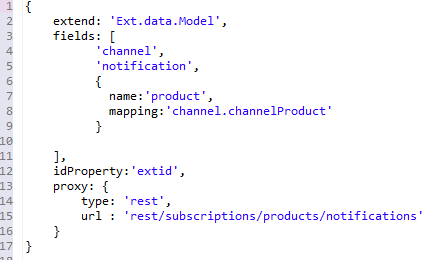
\includegraphics{images/json.png}
	\caption{Przykład użycia formatu JSON}
\end{figure}

\section{Warstwa biznesowa}

Na warstwę biznesową składa się szereg interfejsów pełniących rolę usług. Usługi pozwalają wykonywać wszystkie możliwe operacje na obiektach systemowych. Dzięki takiemu podejściu w~warstwie wyższej, czyli warstwie komunikacji nie trzeba wykonywać żadnych dodatkowych działań. Ponadto, w~momencie pojawienia się potrzeby implementacji systemu na innych platformach, np. PC, systemy mobilne, lub aplikacja oparta o~webservice SOAP, można zastąpić obecną warstwę komunikacji inną, zgodną z~daną platformą bez zmiany niższych warstw.
Interfejsy usług są podzielone w~taki sposób, aby każdy udostępniał szereg operacji z~pewnego logicznie powiązanego zakresu. Implementacja interfejsów nie jest bezpośrednio używana przez warstwę wyższą. Obecnie każdy interfejs implementowany jest przez jedną klasę. Grupa projektowa doszła do wniosku, że interfejsy zapewnią większą elastyczność podczas rozbudowy projektu, oraz ułatwią tworzenie testów jednostkowych.
Implementacja konkretnych usług polega na wykonaniu operacji, które zmienią jeden stan spójny systemu w~drugi. Oznacza to, że wszystkie działania bazodanowe powinny operować na tej samej transakcji w~ramach jednej metody implementującej usługę. W tym miejscu pojawiło się pytanie - jako stworzyć elastyczny mechanizm zarządzania transakcjami bez konieczności umieszczania w~każdej metodzie powtarzającego się schematu otwierającego i~zamykającego transakcję bazodanową. Z~pomocą kolejny raz przychodzi pakiet Spring. Przy minimalnej konfiguracji wystarczy oznaczyć klasę za pomocą @Service, a~metodę implementującą usługę adnotacją @Trasnactional i~można korzystać z~dobrodziejstw transakcji nie martwiąc się o~ich rozpoczęcie i~zakończenie. Wewnątrz metod usług można wywoływać zarówno funkcje interfejsów Repository(warstwa dostępu do danych) jak i~funkcje innych usług, nie podając przy tym jako argumentu obiektu transakcji. Podczas wykonywania operacji bazodanowych menadżer transakcji sprawdza czy w~obecnym wątku istnieje już otwarta transakcja, jeżeli tak to nie otwiera nowej tylko korzysta z~już istniejącej, a~jeżeli nie, to rozpoczyna nową transakcję, która będzie wykorzystywana do momentu wyjścia z~metody, w~której transakcja została utworzona. Jest to oczywiście najprostsza sytuacja, ponieważ adnotacja @Transactional pozwala na bardziej zaawansowane zarządzanie transakcjami. Mechanizm umożliwia nam np. określenie pewnych metod jako wymagających nowej transakcji, lub ustawienie flagi transakcji tylko do odczytu(w celu optymalizacji). Można również określić limit czasu trwania transakcji, oraz dla jakich typów błędów transakcję należy wycofać. 
Kolejną ważną cechą klas usług jest możliwość wywoływania różnych zdarzeń podczas wykonywania operacji. Przykładem wykorzystania tej zalety jest wysyłanie powiadomień o~subskrypcjach recenzentów i~obserwowanych produktach. Wysyłanie powiadomień zostaje uruchomione w~momencie dodania produktu lub recenzji. Wywołanie tych operacji wystarczy dodać tylko w~jednym miejscu projektu.

\section{Warstwa dostępu do danych}

Poza zarządzaniem transakcjami, framework Spring oddaje do naszej dyspozycji technologie, zwalniające programistę z~konieczności implementacji operacji CRUD, a~także znacząco upraszcza implementację bardziej zaawansowanych operacji np. wyszukiwania. Technologie z~których skorzystano do implementacji warstwy dostępu do danych, należą do grupy modułów Spring Data. Projekty te mają na celu uproszczenie i~dostarczenie wsparcia dla obsługi zarządzania różnymi technologiami bazodanowymi, m.in. JPA, MongoDB, Neo4j. W aplikacji RevCommunity wykorzystano projekt dotyczący Neo4j.

Architektura warstwy dostępu do danych składa się z~dwóch głównych elementów. Pierwszym z~nich jest zbiór klas encyjnych, które są mapowane na węzły i~relacje grafowej bazy danych. Drugim jest szereg interfejsów udostępniających operacje bazodanowe. Co ciekawe, podczas pracy nad projektem nie było konieczności implementacji tych interfejsów, ponieważ pakiet Spring Data oferuje standardową implementację podstawowych operacji. Zacznijmy od sposobu mapowania obiektów języka Java na obiekty bazodanowe. Cała konfiguracja opiera się na adnotacjach, dzięki czemu klasy mogą posiadać logikę biznesową, oraz mogą posłużyć jako obiekty wymiany danych między klientem, a~serwerem. Klasy można mapować jako węzły grafu lub jako relacje, w~zależności od ich roli. Do mapowania węzłów używa się adnotacji @NodeEntity, natomiast do mapowania relacji @RelationshipEntity. Wszystkie pola typów prostych tak oznaczonych klas są zapisywane w~bazie danych w~sposób analogiczny do kolumn w~relacyjnych bazach danych. Chcąc zmapować relację między dwoma klasami @NodeEntity należy pole odzwierciedlające powiązanie oznaczyć za pomocą @RelatedTo. Adnotacja ta pozwala zdefiniować nazwę relacji przydatną przy tworzeniu zapytań, oraz kierunek połączenia. Aby pewne powiązania posiadały dodatkowe informacje, zamiast używania @RelatedTo tworzymy nową klasę i~oznaczamy ją adnotacją @RelationshipEntity. W tym przypadku należy oznaczyć przez @StartNode i~@EndNode odpowiednio początkowy i~końcowy węzeł grafu. Dodatkowo każdy węzeł i~każda relacja musi posiadać unikalny identyfikator(zazwyczaj generowany automatycznie) zapisywany do pola oznaczonego przez @GraphId. 

Wstawić schemat bazy danych

Gdy obiekty bazodanowe zostaną zamodelowane, przydatne staną się elementy umożliwiające wykonywanie operacji na tych obiektach. Dlatego stworzono szereg interfejsów pozwalających zarządzać encjami. Do tego celu wykorzystano pakiet Spring Data. Jego zadaniem jest znaczne zredukowanie powtarzającego się kodu implementującego warstwę dostępu do danych. Moduł udostępnia mechanizmy, które w~sposób dynamiczny implementują stworzone przez programistę interfejsy. Aby korzystać z~udogodnień pakietu należy rozszerzyć dostarczony przez Spring Data generyczny interfejs GraphRepository. Jako parametr generyczny podając klasę encji, na której będziemy operować. Od tej chwili można wykonywać podstawowe operacje tj. zapis, odczyt, modyfikacji, czy proste wyszukiwanie. Dodatkowo można dodać do interfejsu definicje metod wykonujących bardziej konkretne zadania poprzez odpowiednią konstrukcję ich nazw. Spring wykorzystuje mechanizm refleksji do wygenerowania zapytania na podstawie nazwy metody, jej parametrów i~definicji klasy, którą przekazano jako parametr generyczny do interfejsu GraphRepository. Spójrzmy na przykład(fragment UserRepo)\cite{repoWww}:

\begin{figure}[H]
	\centering
	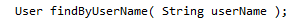
\includegraphics{images/findbyusername.png}
\end{figure}


Powyższa metoda pozwoli pobrać obiekt użytkownika o~podanej nazwie. Mechanizm budujący zapytanie odnajduje wzorzec findBy, po którym występuje nazwa pola klasy, której dotyczy interfejs. Następnie sprawdza, czy argument metody jest tego samego typu, co pole userName klasy User. Jeżeli w~klasie User nie byłoby pola userName lub jego typ nie zgadzałby się z~typem argumentu, to podczas uruchamiania systemu rzucony zostałby wyjątek. 
Nazwy metod mogą wykorzystywać bardziej złożone wzorce, pozwalające na zdefiniowanie wielu pól po których chcemy wyszukiwać. Warunki dotyczące pól można łączyć operatorami logicznymi AND i~OR.  Można również ustawić pewne opcje dodatkowe tj. ignorowanie wielkości znaków, czy usunięcie duplikatów ze zbioru wyników. Suffix Asc lub Desc określa sortowanie elementów. Bardziej rozbudowany przykład mógłby wyglądać następująco:

\begin{figure}[H]
	\centering
	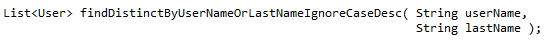
\includegraphics{images/findlong.png}
\end{figure}


Taka metoda wygeneruje zapytanie pobierające użytkowników o~podanym loginie lub nazwisku, z~wykluczeniem duplikatów(słowo distinct) posortowanych malejąco i~przy porównywaniu nazwiska zostanie pominięta wielkość znaków. 
Poza tworzeniem zapytań poprzez nazwy metod można również wykorzystać natywne zapytanie bazodanowe. Co prawda, takie podejście bardziej uzależnia aplikację od wybranej technologii, jednak w~tym przypadku system bazuje na zapytaniach korzystających ze specyficznych możliwości grafowej bazy danych. Metody wykonujące zapytania również można umieszczać w~definicji interfejsu. Jedną rzeczą, która należy wykonać, jest oznaczenie metody adnotacją @Query i~wpisanie w~niej treść zapytania. Do zapytania możemy oczywiście wprowadzać parametry, które zostaną pobrane z~definicji metody. Językiem w~którym będziemy komunikować się z~bazą danych Neo4j jest Cypher. 

Przejdźmy do przykładu:

\begin{figure}[H]
	\centering
	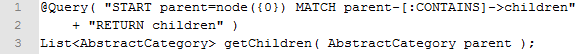
\includegraphics{images/query.png}
\end{figure}

Jako parametr podano kategorię, dla której należy znaleźć kategorie podrzędne(dzieci). Podany argument jest miejscem zaczepienia w~grafie, od którego rozpocznie się dopasowanie. Klauzula MATCH odpowiada za definicje relacji między węzłami biorącymi udział w~dopasowaniu. Słowo kluczowe RETURN określa, który ze zdefiniowanych elementów zostanie zwrócony jako wynik zapytania. Najciekawsza tutaj jest klauzula MATCH. To ona wprowadza abstrakcję grafu i~odróżnia zapytanie od np. języka SQL. Fragment zawarty między MATCH, a~RETURN określa wzór dopasowania między węzłem parent(podanym jako parametr) a~węzłami połączonymi z~nim jednokierunkową wychodzącą relacją o~nazwie CONTAINS. 

\section{Import danych z~zewnetrznych serwisow przy pomocy udostepnionego API}

Stworzona aplikacja umożliwia import informacji o~kategoriach i~produktach z~zewnętrznych serwisów przy pomocy udostępnianego przez nie API (ang. \textit{Application Programming Interface}). Import danych odbywa się przy pomocy stworzonego interfejsu \textit{RemoteService}. Interfejs ten implementują dwie usługi, \textit{AllegroService} oraz \textit{NokautService}.

\begin{figure}[h]
	\centering
	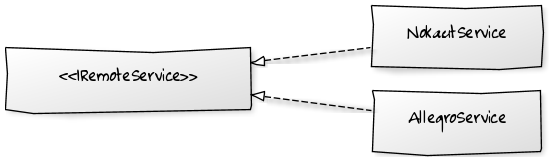
\includegraphics[scale=1]{images/uml_remote_service2.png}
	\caption{Diagram UML przedstawiający powiązanie między obiektami.}
\end{figure}

Pierwsza z~nich umożliwia import opisanych wcześniej informacji z~serwisu Allegro przy pomocy SOAP(ang. \textit{Simple Object Accesss Protocol}).SOAP jest protokołem umożliwiającym zdalne wykonywanie udostępnionych usług. Komunikacja polega na przesyłaniu pliku XML w~odpowiednim formacie, który może zawierać żądanie wykonania określonej usługi lub odpowiedź dotyczącą wykonanej usługi.\cite{soap} \indent Druga natomiast do pozyskiwania informacji z~portalu nokaut.pl, wykorzystuje wzorzec REST(ang. \textit{Representational State Transfer}) oraz klucz autoryzujący.

\subsection{API Allegro}
API udostępnione przez Allegro, jest bardzo rozbudowane i~umożliwia pozyskanie wielu przydatnych informacji, np. drzewo kategorii, zestaw filtrów dla każdej z~kategorii oraz informacje o~wygranych aukcjach.
Podczas tworzenia aplikacji okazało się, że API serwisu Allegro nie spełnia w~zupełności naszych potrzeb.
Nie udostępnia wszystkich potrzebnych danych, wykorzystywanych przez system RevCommunity. Przede wszystkim w~serwisie Allegro nie istnieje obiekt typu produkt. Dostępne są jedynie aukcje, które nie gwarantują występowania unikalnych informacji o~produktach. Współpraca z~tym API wymagałaby po stronie RevCommunity odfiltrowania aukcji dotyczących powtarzających się produktów, co jest czasochłonne i~nie gwarantuje całkowitej skuteczności. Z~tego względu współpraca z~tym API nie była kontynuowana.

\subsection{API Nokaut.pl}
Dostęp do API serwisu nokaut.pl, jest możliwy przy pomocy klucza autoryzującego. Aby uzyskać klucz należało:
\begin{itemize}
\item Zgłosić się do programu partnerskiego portalu
\item Zaakceptować regulamin programu partnerskiego, który między innymi obliguje do zamieszczenia linków do nokaut.pl, na każdej stronie, na której znajdują się informacje pobrane przy jego pomocy
\item Wysłać wiadomość na podany adres skrzynki emailowej, z~informacją dotyczącą celu wykorzystania API
\end{itemize}
Po pozytywnym rozpatrzeniu prośby, w~zwrotnej wiadomości email został zawarty wygenerowany klucz autoryzujący.

API portalu nokaut.pl, dostarcza więcej przydatnych informacji w~porównaniu z~tym udostępnianym przez Allegro. Przy jego pomocy mamy możliwość pobrania następujących informacji:

\begin{itemize}
\item Pełne drzewo kategorii
\item Filtry dla poszczególnych kategorii
\item Unikalnych produktów
\end{itemize}

Komplet niezbędnych danych uzyskaliśmy poprzez dodatkowe parsowanie strony internetowej w~portalu nokaut.pl, na której znajduje się opis produktu. Parsowanie polegało na pozyskiwaniu informacji z~kodu źródłowego strony HTML(ang. \textit{HyperText Markup Language}). Uzyskane informacje zawierały między innymi, nazwę producenta, opis produktu oraz jego specyfikację. Taki zbiór informacji stanowi wystarczającą bazę danych, potrzebną do automatycznego wygenerowania danych w~systemie.

\section{Zabezpieczenia, model uprawnień}

Dostęp do systemu RevCommunity został zabezpieczony przy użyciu platformy Spring Security. Platforma ta umożliwia uwierzytelnianie oraz autoryzację użytkowników w~systemie. Dodatkowo Spring Security umożliwia modelowanie uprawnień dla grup zdefiniowanych w~systemie.

\begin{figure}[H]
	\centering
	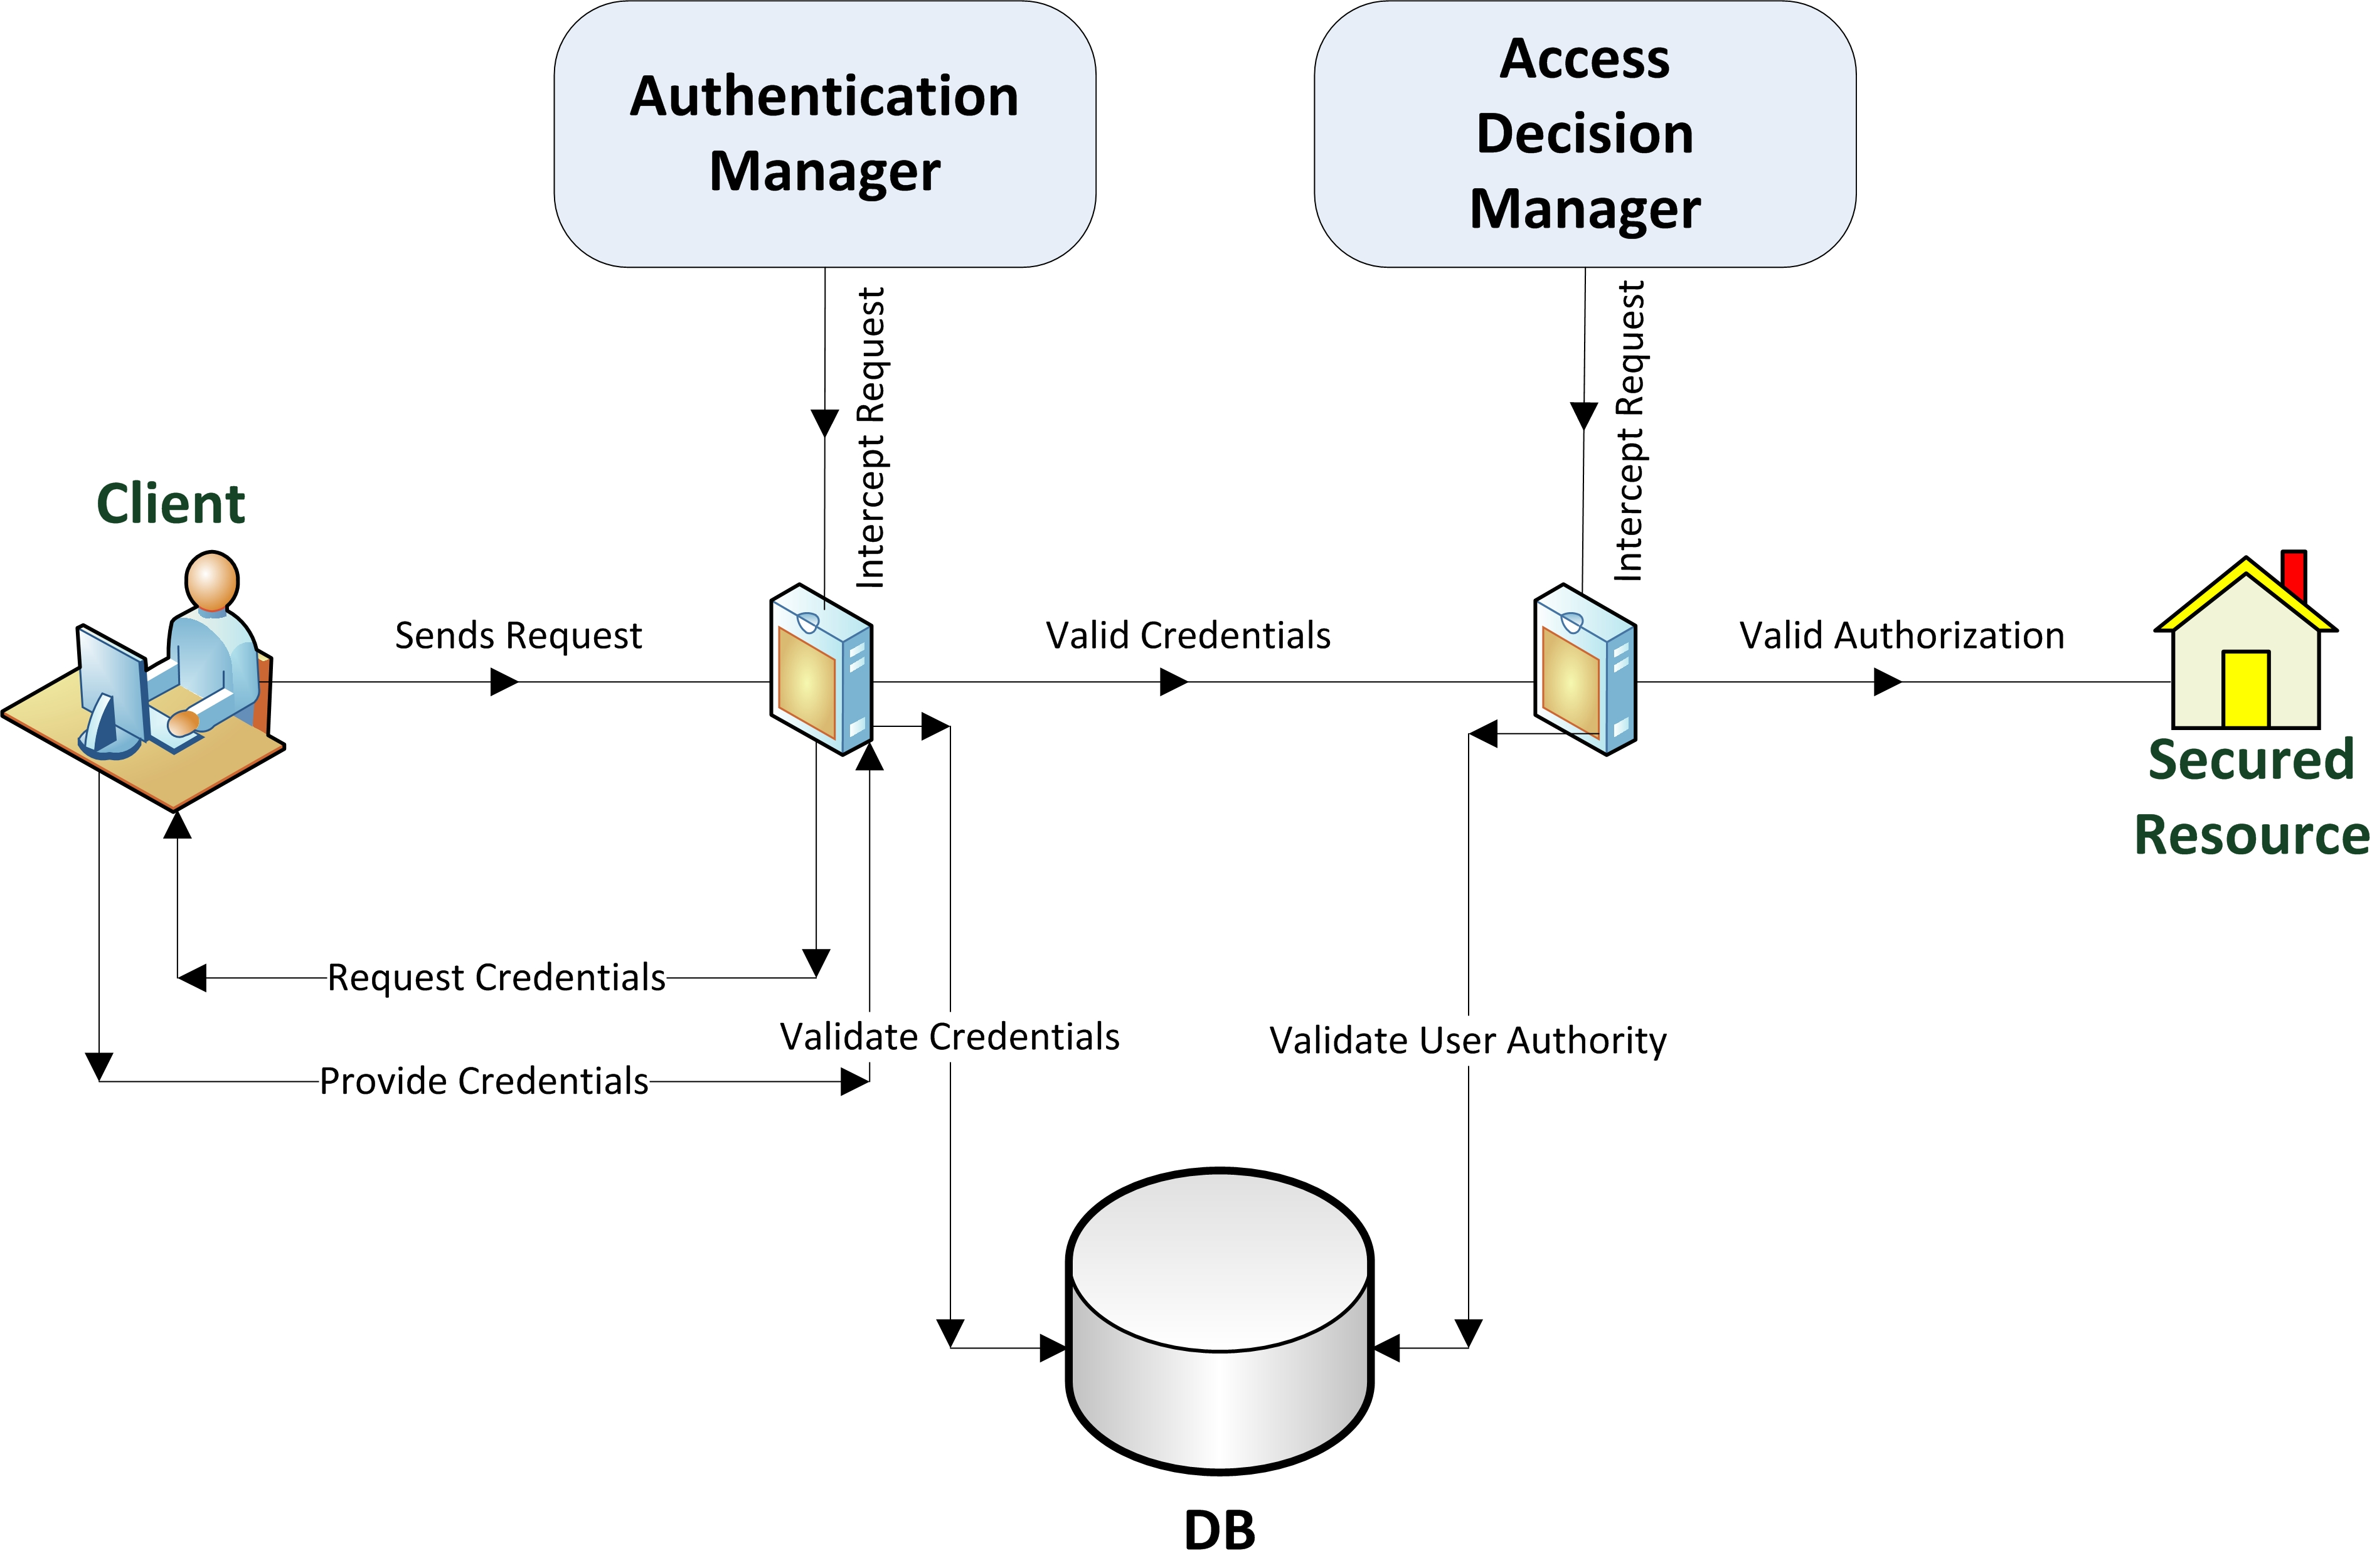
\includegraphics[width=1.00\textwidth]{images/spring_diagram.jpg}
	\caption{Schemat procedury uwierzytelnienia oraz autoryzacji w~platformie Spring Security.}
\end{figure}

Proces uwierzytelnienia polega na weryfikacji nazwy oraz hasła konta użytkownika zarejestrowanego w~systemie, w~celu potwierdzenia jego tożsamości. 

Proces autoryzacji z~kolei ma na celu weryfikację czy dany użytkownik ma dostęp do żądanego zasobu systemowego. Po wysłaniu żądania przez klienta, platforma Spring Security sprawdza do jakiej grupy użytkownik jest przypisany. Na podstawie tej informacji oraz zdefiniowanego modelu uprawnień jest przyznawany lub nie, dostęp do żądanego zasobu.

\subsection{Model uprawnień}

Model uprawnień został zdefiniowany w~pliku konfiguracyjnym SpringSecurity. Zawiera on definicję uprawnień dla  trzech grup użytkowników:

\begin{itemize}
\item Anonimowych
\item Zarejestrowanych w~systemie
\item Administratorów
\end{itemize}

\begin{figure}[h]
	\centering
	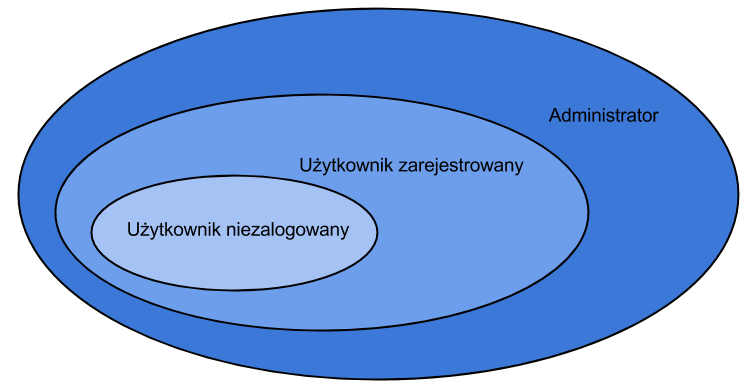
\includegraphics[width=1.00\textwidth]{images/hierarchia_uprawnien.png}
	\caption{Hierarchia uprawnień pomiędzy użytkownikami.}
\end{figure}

Na diagramie widać, że uprawnienia są dziedziczone. Użytkownicy niezalogowani posiadają swoją określoną pulę uprawnień. Użytkownicy zarejestrowani posiadają tą samą grupę uprawnień co użytkownicy nie zalogowani oraz dodatkową pule uprawnień nie dostępną dla użytkowników nie zarejestrowanych. Przykładem takiego uprawnienia może być między inny możliwość dodawania i~oceniania recenzji. Administrator natomiast posiada wszystkie uprawnienia dostępne w~systemie. Dodatkowymi możliwościami w~przypadku administratora, które nie są dostępne dla zarejestrowanego użytkownika, są między innymi:

\begin{itemize}
\item Dodawanie nowego produktu
\item Dodawanie nowej kategorii
\item Uruchomienie importu danych z~zewnętrznego serwisu
\end{itemize}

\begin{figure}[h]
	\centering
	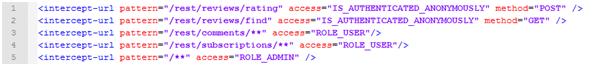
\includegraphics[width=1.00\textwidth]{images/model_uprawnien_xml.png}
	\caption{Przykładowe wpisy zawarte w~pliku konfiguracyjnym.}
\end{figure}

Powyższy fragment pliku konfiguracyjnego przedstawia uprawnienia do poszczególnych zasobów przez istniejące w~systemie grupy użytkowników. Znaczenie poszczególnych grup:

\begin{itemize}
\item IS\_AUTHENTICATED\_ANONYMOUSLY – użytkownicy nie posiadający konta w~systemie
\item ROLE\_USER – użytkownicy posiadający zarejestrowane kont w~systemie
\item ROLE\_ADMIN – użytkownicy pełniący rolę administratorów
\end{itemize}

 Zapis w~pierwszej oraz drugiej linii oznacza że użytkownicy nie zarejestrowani mają dostęp do usług, które umożliwiają pobranie informacji o~recenzjach istniejących w~systemie oraz ich ocenach.
Kolejne dwie linie (3 oraz 4) dotyczą użytkowników zarejestrowanych. Oznaczają one, że ci użytkownicy mają dostęp do wszystkich zasobów oraz usług, które są związane z~komentarzami oraz subskrypcjami.
Ostatnia linia (linia numer 5), definiuje uprawnienia użytkowników należących do grupy administratorów. Oznacza ona, że mają oni dostęp do wszystkich zasobów i~usług serwisu.

Przedstawione nazwy grup, są grupami domyślnymi w~platformie Spring Security. Oznacza to, że nie musimy definiować dziedziczenia uprawnień pomiędzy nimi. Domyślnie grupa ROLE\_USER dziedziczy uprawnienia grupy \newline IS\_AUTHENTICATED\_ANONYMOUSLY, natomiast ROLE\_ADMIN, dziedziczy uprawnienia z~ROLE\_USER.\cite{springSecurity}

\subsection{Zabezpieczenie komunikacji}

Komunikacja pomiędzy klientem a~serwerem odbywa się przy pomocy protokołu TLS w~wersji 1.2. Dzięki zastosowaniu tego protokołu, zapewniona jest poufność oraz integralność przesyłanych informacji, zwłaszcza nazwy oraz hasła użytkownika, pomiędzy klientem a~serwerem. Poufność komunikacji odbywa się poprzez szyfrowanie przesyłanych informacji. Szyfrowanie wiadomości chroni ją przed nieautoryzowanym dostępem do jej zawartości przez osoby trzecie.
Integralność informacji przesyłanych pomiędzy klientem a~serwerem jest natomiast zapewniona dzięki podpisowi cyfrowemu dołączanemu do wiadomości. Gwarantuje to, że informacje przesyłane pomiędzy klientem, a~serwerem, nie zostały zmodyfikowane w~trakcie transmisji.
 Protokół TLS umożliwia także weryfikację tożsamości serwera. Polega to na sprawdzeniu czy serwer posiada poprawny certyfikat, przy pomocy, którego potwierdza swoją autentyczność. O autentyczności serwisu świadczy certyfikat, który jest przedstawiany klientowi. Tego typu certyfikat pozyskiwany jest od zaufanego organu certyfikującego. Klient widząc certyfikat podpisany przez zaufany urząd certyfikujący, ma pewność, że nawiązuje połączenie z~prawdziwym serwerem.\cite{tls}
\paragraph{}
Przy tym zestawie zabezpieczeń użytkownik może swobodnie i~bezpiecznie korzystać z~usług oraz zasobów serwisu RevCommunity.
